\section{Probability}\label{section:probability}
This section is regarding probability, specifically forward propagation.
The concept of probability in machine intelligence is to make a decision based on observations of a domain.
The information, which is used for calculating probability can be discrete or continuous. 
In this project the primary focus will be on continuous variables, however discrete variables will be briefly explained.

\subsection{Discrete Variables}\label{subsection:discrete-variables}
In probability, $\Omega$ is used to describe the set of possible worlds, which contains all the states or variables in that space, e.g. all the possible numbers a dice can roll $(\Omega = \{1, 2, 3, 4, 5, 6\})$, which is a finite set.
The probability space, written $P(a)$, is the probability of some variable or event, e.g. the probability of rolling even numbers with a dice $P(even = true) = P(2) + P(4) + P(6) = 3/6$. 
There can be a proposition for an event, where the proposition can either be true or false, e.g a six-sided dice can have the following proposition:
$$P(dice) = one_{eye} \vee two_{eye} \vee three_{eye} \vee four_{eye} \vee five_{eye} \vee six_{eye}$$
It is possible to find the probability of an event given that another event has occurred, which have an effect on the state space.
It is called conditional probability and is denoted by $P(A|B)$ which can be translated as \textit{the probability of A given B}.
Sometimes these event are independent meaning that they do not affect each other, e.g. the outcome of a new roll, is not affected by the previous roll.
To find the probability distribution, the 
Gaussian distribution is used to find the probability around a given point.
The distribution can be used to find the probability between two numbers by integrating the Gaussian distribution function.

\subsection{Continuous Variables}\label{subsection:continuous-variables}
The properties of continuous variables are described in \secref{section:bayesian-network}.
Probability for continuous variables is different from discrete variables, as the set of possible worlds $\Omega$ = $\{\mathbb{R}\}$, which is not a finite set. 
The probability for a continuous random variable X can be written as $P(a \leq X \leq b)$, where a and b are exact numbers.
The probability can be calculated in different ways, one of which is a probability density function.

For continuous variables the continuous probability density function can be calculated by taking the integral of the density function. 
It is defined as:
\begin{equation}
\int\limits_{a}^{b} f(x)dx 
\end{equation}
where $a$ and $b$ determines the interval of the integral. 
If $a = -\infty$ and $b = \infty$, the integral of the graph will have a probability of 1.

A simple example for using continuous variables is finding the probability for the amount of rain that will fall tomorrow, $P(Y)$. 
A function for the rain fallen, $f(x)$, could be shown as in \figref{figure:pdf-graph}.
The probability for this could be described as an interval:
$P(1.5 \le Y \le 2.5)$

From the graph, it can be seen that the probability of the amount of rain, that will fall tomorrow, is more likely to be between numbers 1.5 and 2.5 rather than between 3 and 4.
The exact probability for this can be found by using the integral of function $f(x)$:
$\int\limits_{1.5}^{2.5} f(x)dx$.

\begin{figure}[h]
	\centering
	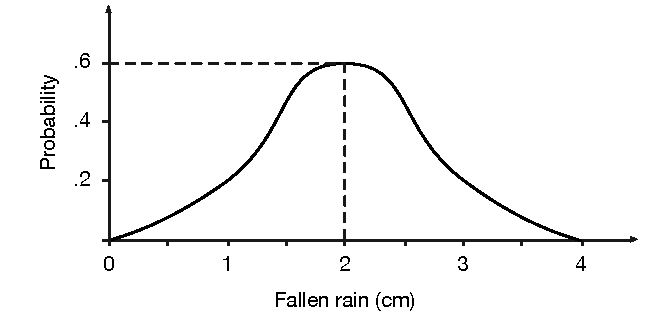
\includegraphics[scale = 0.7]{media/Theory/probability-density-function}
	\caption{A probability distribution over how much rain has fallen.}
	\label{figure:pdf-graph}
\end{figure}